\chapter{Explotación}

En este capítulo se expone la explotación del simulador de escenarios como método para la evaluación de sistemas de recomendaciones, se expone el trabajo realizado para permitirlo y el rendimiento obtenido del simulador.

\section{Motivación}

Debido a la gran cantidad de información resulta difícil para los usuarios elegir entre todas las alternativas existentes en los resultados mostrados por un sistema. Por ello, para facilitar la elección se utilizan los llamados sistemas de recomendación. Estos sistemas resultan de gran interés para las empresas desde punto de vista económico, ya que hacen llegar a sus cliente recomendaciones de productos relevantes para ellos. Ademas, también resultan de interés para los usuarios ya que actúan como filtro y les ofrecen información personalizada que les resulta de interés.

No obstante, el diseño de sistemas de recomendación se enfrenta a problema como el arranque en frió (cold
start problem) o el problema de opiniones artificiales o manipuladas (spam). Esto conlleva que el sistema de recomendación muestra información no relevante para el usuario y este dejará de confiar en él y abandonarlo. 

Por esto surge la necesidad de que los sistemas de recomendaciones puedan evaluarse y calibrarse correctamente. Para que esto pueda llevarse a cabo necesitamos recolectar datos reales de escenarios reales para su posterior análisis. Este análisis consiste en calcular el error cometido por el sistema de recomendación. Una forma de cuantificar el error es con la MAE (Medium Absolute Error) que consiste en restar el valor asignado por el usuario del valor estimado por el sistema de recomendación. 

\section{Definir un escenario realista}

En este apartado se expone como definir un escenario realista con datos de restaurantes reales de la ciudad San Luis Potosí de México.

\subsection{Paso 1: obtener datos de restaurantes reales}

Lo primero que vamos a hacer es conseguir datos reales de restaurantes reales. Por esto accedemos al repositorio de Center for Machine Learning and Intelligent Systems y descargamos el siguiente archivo comprimido: \href{https://archive.ics.uci.edu/ml/machine-learning-databases/00232/RCdata.zip}{https://archive.ics.uci.edu/ml/machine-learning-databases/00232/RCdata.zip}

Una vez que hayamos descargado y descomprimido el fichero vemos que este contiene varios ficheros csv. A nosotros nos interesan los ficheros geoplaces2.csv y rating\_final.csv. El primero contiene los datos de los restaurantes y es el que vamos a importar al crea un escenario y el segundo contiene datos con valoraciones de diferentes usuarios y el que vamos a usar como datos de entrenamiento para el recomendador de ejemplo desarrollado.

\subsection{Paso 2: crear un mapa nuevo o editar un mapa existente}

Antes de todos tenemos que crear un mapa nuevo o editar uno existente para poder asociarle el escenario que vamos a crear a continuación. Por esto tenemos que usar alguna de las dos opciones:
\begin{itemize}
	\item crear un mapa nuevo: opción  Maps $\rightarrow$ new map. Para más información por favor consulte el anexo \ref{sec:crearMapa}.
	\item editar un mapa existente: opción Maps $\rightarrow$ maps search y en la lista de resultados pulsamos sobre el icono de editar imagen. Para más información por favor consulte el anexo \ref{sec:editarMapasEscenas}.
\end{itemize} 

En este caso se ha optado por crear un nuevo mapa con el nombre México ya que los datos que hemos descargado son de la ciudad San Luis Potosí de México. En la figura \ref{mapaMexico} podemos ver una captura del resultado de creación del mapa:

\begin{figure}[H]
	\centering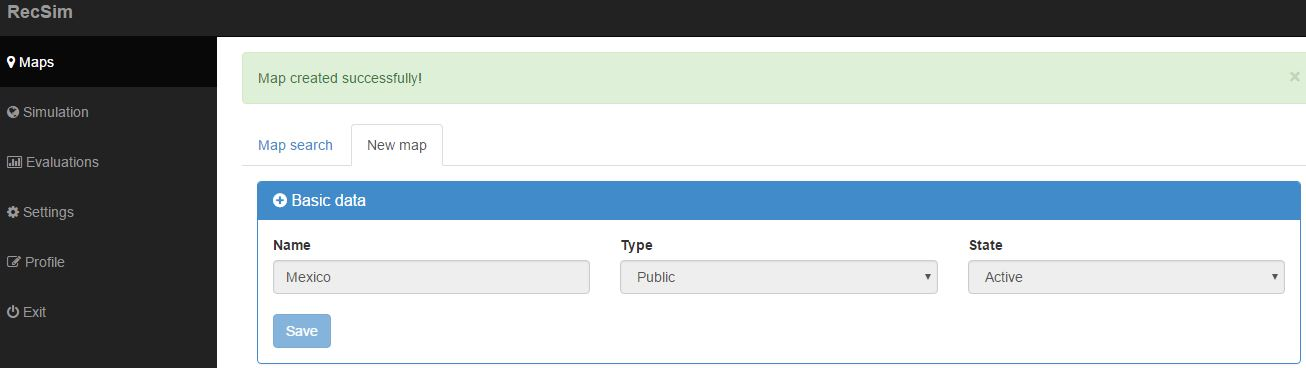
\includegraphics[scale=0.36]{imagenes/crear-mapa-nuevo-mexico.jpg}
	\caption{Creación de un mapa nuevo en México con datos reales}
	\label{mapaMexico}
\end{figure}

\subsection{Paso 3: crear un escenario realista}

La creación de escenarios funciona como un asistente de configuración. A continuación se muestra los pasos que hay que realizar para configurar un escenario realista:

\subsubsection{Paso 3.1: definir el nombre del escenario y elegir el recomendador}


\subsubsection{Paso 3.2: definir los limites del escenario}


\subsubsection{Paso 3.3: importar los datos de los restaurantes}



\subsubsection{Paso 3.4: definir los objetos móviles}


\section{Realizar una simulación de un escenario realista}


\section{Evaluación de un sistema de recomendación}



\section{Rendimiento}


